\documentclass[12pt]{article}
%\documentclass{amsart}
\usepackage{pstricks}
\usepackage{graphicx}
%\usepackage[margin=2in,showframe=true]{geometry}
\usepackage{amssymb,amsfonts,amsmath,mathtools,tensor}
\usepackage[alphabetic,y2k,lite]{amsrefs}
%\usepackage{fullpage, mystyle}
\usepackage{markdown}
\usepackage{MnSymbol}
\usepackage{xcolor}
%\usepackage{cite}
%\usepackage[english]{babel}
%%%%%%%%%%%%%%%%%% Tikz %%%%%%%%%
\usepackage{tikz}
\usetikzlibrary{shapes.geometric, arrows}
\usetikzlibrary{shapes.multipart} %% for multiple lines in node (must have align=center)
\usetikzlibrary{scopes}
\usetikzlibrary{math}
\usetikzlibrary{decorations.markings,decorations.pathreplacing}
\usetikzlibrary{fadings}
\usepackage{tikz-cd}

\tikzset{
every picture/.style={line width=0.8pt, >=stealth,
                       baseline=-3pt,label distance=-3pt},
%%%%%%%%%%  Node styles
emptynode/.style={circle,minimum size=0pt, inner sep=0pt, outer
sep=0},
dotnode/.style={fill=black,circle,minimum size=2.5pt, inner sep=1pt, outer
sep=0},
small_dotnode/.style={fill=black,circle,minimum size=2pt, inner sep=0pt, outer
sep=0},
morphism/.style={fill=white,circle,draw,thin, inner sep=1pt, minimum size=15pt,
                 scale=0.8},
small_morphism/.style={fill=white,circle,draw,thin,inner sep=1pt,
                       minimum size=10pt, scale=0.8},
ellipse_morphism/.style args={#1}{fill=white,circle,draw,thin,inner sep=1pt,
                       minimum size=5pt, scale=0.8,
												ellipse, draw, rotate=#1},
%note that ellipse stretches based on the text inside, so put \;\;\; in label
coupon/.style={draw,thin, inner sep=1pt, minimum size=18pt,scale=0.8},
semi_morphism/.style args={#1,#2}{
                  fill=white,semicircle,draw,thin, inner sep=1pt, scale=0.8,
                  shape border rotate=#1,
                  label={#1-90:#2}},
%%can only rotate semi_morphisms by right angles tho
%%%% different line styles:
regular/.style={densely dashed}, %% for the regular color, i.e. sum d_i
edge/.style={very thick, draw=green, text=black},
overline/.style={preaction={draw,line width=2mm,white,-}},
thin_overline/.style={preaction={draw,line width=#1 mm,white,-}},
thin_overline/.default=2,
thick_overline/.style={preaction={draw,line width=3mm,white,-}},
really_thick/.style={line width=3mm, gray},
%drinfeld center/.style={>=stealth,green!60!black, double
%distance=1pt,text=black},
boundary/.style={thick,  draw=blue, text=black},
%arrow_decoration={markings, mark=at position 0.5 with {\arrow{>}}}
ribbon/.style={line width=1.5mm, postaction={draw,line width=1mm,white}},
ribbon_u/.style args={#1,#2}{line width=#1mm, postaction={draw,line width=#2mm,white}},
%use line width=0.4pt for thin lines to point to things
%%%%%%% Fill styles %%%%%%%%%%%%%%%
cell/.style={fill=black!10},
subgraph/.style={fill=black!30},
%%%%%%% Mid-path arrows
midarrow/.style={postaction={decorate},
                 decoration={
                    markings,% switch on markings
                    mark=at position #1 with {\arrow{>}},
                 }},
midarrow/.default=0.5,
%%%%% Mid-path arrow but reverse
midarrow_rev/.style={postaction={decorate},
                 decoration={
                    markings,% switch on markings
                    mark=at position #1 with {\arrow{<}},
                 }},
midarrow_rev/.default=0.5,
%%%%% for the flowchart; need align=center to allow multiline in node
block/.style={rectangle, rounded corners, text centered, draw=black, align=center}
}

%% style for flow chart blocks
\tikzstyle{block} = [rectangle, rounded corners, text centered, draw=black, align=center]

%% for shading with gradients
\tikzfading[name=fade inside, inner color=transparent!80, outer
color=transparent!10]


\begin{document}

%%%%%%%%%%%%%%%%%%%%%%%%%%%%%%%%%%%%%%%%%%%%%%%%%%%%%%%%%%%%%%%%%%%%%
%graphic 01
%\begin{tikzpicture}
%\draw[->] (0,0.7) -- (2.2,0.7)
%	node[pos=0,left] {$i$} node[pos=1,right] {$i$};
%\draw[->] (0,0) -- (2.2,0)
%	node[pos=0,left] {$X$} node[pos=1,right] {$X$};
%\node[dotnode] (a) at (0.8,0) {};
%\node[emptynode] (b) at (0.6,1) {};
%\node[emptynode] (c) at (1.3,0.7) {};
%\node[emptynode] (d) at (1.4,-0.3) {};
%\draw[overline,regular] (a) .. controls +(120:1cm) and +(180:0.2cm) ..
%	(b) .. controls +(0:0.2cm) and +(120:0.4cm) ..
%	(c) .. controls +(-60:1cm) and +(0:0.2cm) ..
%	(d) .. controls +(180:0.2cm) and +(-60:0.4cm) .. (a);
%\draw[overline] (1,0.7) -- (2,0.7);
%\draw[overline] (1,0) -- (2,0);
%%%some labels
%\node at (0.6,-0.2) {\small $\gamma$};
%\node at (0.9,1.2) {\small $\Omega$};
%\end{tikzpicture}
%%%%%%%%%%%%%%%%%%%%%%%%%%%%%%%%%%%%%%%%%%%%%%%%%%%%%%%%%%%%%%%%%%%%%%
%
%
%
%%%%%%%%%%%%%%%%%%%%%%%%%%%%%%%%%%%%%%%%%%%%%%%%%%%%%%%%%%%%%%%%%%%%%%
%graphic 02
%\begin{tikzpicture}
%%%left right columns
%\node (y) at (0,0) {$Y$};
%\node at (0,0.8) {$\boxtimes$};
%\node (x) at (0,1.6) {$X$};
%\node (I) at (4.5,0) {$I_{i_* F(X \boxtimes Y)}$};
%\node at (4,0.8) {$\boxtimes$};
%\node (i8) at (4,1.6) {$i^*$};
%%%middle column
%\node (y2) at (2,-0.8) {\small $Y$};
%\node at (2,-0.4) {\small $\otimes$};
%\node (x2) at (2,0) {\small $X$};
%\node at (2,0.4) {\small $\otimes$};
%\node (i) at (2,0.8) {\small $i$};
%%%lines
%\draw[->] (x) -- (i8)
%	node[pos=0.5,above] {\small $\alpha_{i,k}$};
%\draw[->] (y) to[out=-20,in=180] (y2);
%\draw[->>] (2.8,0) -- (I);
%\draw[decorate,decoration={brace,amplitude=6pt,mirror,raise=2pt}]
%	(2.3,-0.8) -- (2.3,0.8);
%%coev
%\draw %[midarrow_rev={0.3}]
%	(i) .. controls +(-170:1.2cm) and +(170:1.2cm) .. (x2);
%\node[dotnode] at (1.3,0.15) {};
%\node at (1.3,-0.1) {\tiny $\alpha_i^k$};
%\node[dotnode] at (1.05,0.4) {};
%\node at (0.7,0.4) {\tiny coev};
%\end{tikzpicture}
%%%%%%%%%%%%%%%%%%%%%%%%%%%%%%%%%%%%%%%%%%%%%%%%%%%%%%%%%%%%%%%%%%%%%%
%
%
%
%%%%%%%%%%%%%%%%%%%%%%%%%%%%%%%%%%%%%%%%%%%%%%%%%%%%%%%%%%%%%%%%%%%%%%
%graphic 03
%\begin{tikzpicture}
%%%left right columns
%\node (y) at (4,0) {$Y$};
%\node at (4,0.8) {$\boxtimes$};
%\node (x) at (4,1.6) {$X$};
%\node (I) at (0,0) {$I_{i_* F(X \boxtimes Y)}$};
%\node at (0,0.8) {$\boxtimes$};
%\node (i8) at (0,1.6) {$i^*$};
%%%middle column
%\node (y2) at (2,-0.8) {\small $Y$};
%\node at (2,-0.4) {\small $\otimes$};
%\node (x2) at (2,0) {\small $X$};
%\node at (2,0.4) {\small $\otimes$};
%\node (i) at (2,0.8) {\small $i$};
%%%lines
%\node at (1.1,0) {$\subseteq$};
%\draw[->] (y2) to[out=0,in=-160] (y);
%\draw[->] (i8) -- (x)
%	node[pos=0.5,above] {\small $\alpha_i^k$};
%\draw[decorate,decoration={brace,amplitude=6pt,raise=2pt}]
%	(1.7,-0.8) -- (1.7,0.8);
%%ev
%\draw (x2) .. controls +(10:1.2cm) and +(-10:1.2cm) .. (i);
%\node[dotnode] at (2.75,0.18) {};
%\node at (2.8,-0.05) {\tiny $\alpha_{i,k}$};
%\node[dotnode] at (2.95,0.4) {};
%\node at (3.2,0.4) {\tiny ev};
%\end{tikzpicture}
%%%%%%%%%%%%%%%%%%%%%%%%%%%%%%%%%%%%%%%%%%%%%%%%%%%%%%%%%%%%%%%%%%%%%%
%
%
%%%%%%%%%%%%%%%%%%%%%%%%%%%%%%%%%%%%%%%%%%%%%%%%%%%%%%%%%%%%%%%%%%%%%%
%graphic 04
%\begin{tikzpicture}
%%%left right column
%\node (x) at (0,-0.8) {$X$};
%\node (I) at (5.3,-0.4) {$I_{i,(X,\gamma)}$};
%\node (i82) at (5,0.8) {$i^*$};
%\node at (5,0.2) {$\otimes$};
%%%middle column
%\node (x2) at (2,-0.8) {$X$};
%\node at (2,-0.4) {$\otimes$};
%\node (i) at (2,0) {$i$};
%\node at (2,0.4) {$\otimes$};
%\node (i8) at (2,0.8) {$i^*$};
%%%lines
%\draw[->] (x) -- (x2);
%\draw[->] (i8) -- (i82);
%\draw[->] (2.8,-0.4) -- (I)
%	node[pos=0.5,below] {\tiny $(\twoheadrightarrow) \circ \Gamma_{i,(X,\gamma)}$};
%\draw[decorate,decoration={brace,amplitude=6pt,mirror,raise=2pt}]
%	(2.3,-0.8) -- (2.3,0);
%%coev
%\node[dotnode] (coev) at (1,0.4) {};
%\node at (0.6,0.4) {\tiny coev};
%\draw (coev) to[out=70,in=180] (i8);
%\draw (coev) to[out=-70,in=180] (i);
%\end{tikzpicture}
%%%%%%%%%%%%%%%%%%%%%%%%%%%%%%%%%%%%%%%%%%%%%%%%%%%%%%%%%%%%%%%%%%%%%%
%
%
%%%%%%%%%%%%%%%%%%%%%%%%%%%%%%%%%%%%%%%%%%%%%%%%%%%%%%%%%%%%%%%%%%%%%%
%graphic 05
%\begin{tikzpicture}
%%%left right column
%\node (x) at (5,-0.8) {$X$};
%\node (I) at (0,-0.4) {$I_{i,(X,\gamma)}$};
%\node (i82) at (0,0.8) {$i^*$};
%\node at (0,0.2) {$\otimes$};
%%%middle column
%\node (x2) at (3,-0.8) {$X$};
%\node at (3,-0.4) {$\otimes$};
%\node (i) at (3,0) {$i$};
%\node at (3,0.4) {$\otimes$};
%\node (i8) at (3,0.8) {$i^*$};
%%%lines
%\draw[->] (x2) -- (x);
%\draw[->] (i82) -- (i8);
%\draw[->] (I) -- (2.2,-0.4)
%	node[pos=0.5,below] {\tiny $\Gamma_{i,(X,\gamma)} \circ \subseteq$};
%\draw[decorate,decoration={brace,amplitude=6pt,raise=2pt}]
%	(2.7,-0.8) -- (2.7,0);
%%coev
%\node[dotnode] (ev) at (4,0.4) {};
%\node at (4.3,0.4) {\tiny ev};
%\draw (ev) to[out=110,in=0] (i8);
%\draw (ev) to[out=-110,in=0] (i);
%\end{tikzpicture}
%%%%%%%%%%%%%%%%%%%%%%%%%%%%%%%%%%%%%%%%%%%%%%%%%%%%%%%%%%%%%%%%%%%%%%%
%
%
%%%%%%%%%%%%%%%%%%%%%%%%%%%%%%%%%%%%%%%%%%%%%%%%%%%%%%%%%%%%%%%%%%%%%%%
%graphic 06
%\begin{tikzpicture}
%\begin{scope}[shift={(0,0)}]
%%%cross strand
%\node[emptynode] (e) at (0.6,0.7) {};
%\draw[->] (-2,1.6)
%	.. controls +(0:2cm) and +(120:0.5cm) .. (e)
%	.. controls +(-60:0.5cm) and +(180:0.5cm) .. (2,-1)
%	node[pos=1,right] {$Z$};
%%%X and coev
%\draw[->,overline] (-2,0) -- (2,0)
%	node[pos=1,right] {$X$};
%\draw[->,overline] (0,0.5) -- (2,0.5)
%	node[pos=1,right] {$i$};
%\draw[overline] (0,0.5)
%	.. controls +(180:0.8cm) and +(180:0.8cm) .. (0,1);
%\draw[overline] (0,1) -- (2,1);
%%%omega
%\node[dotnode] (ga) at (0,0) {};
%\node at (-0.15,-0.15) {\tiny $\gamma$};
%\node[emptynode] (a) at (0.2,0.5) {};
%\draw[overline,regular] (ga)
%	.. controls +(120:0.8cm) and +(120:0.5cm) .. (a)
%	.. controls +(-60:0.8cm) and +(-60:0.5cm) .. (ga);
%%%over
%\draw[overline] (0.2,0) -- (1,0);
%\draw[overline] (0,0.5) -- (1,0.5);
%\draw[overline] (-2,1.6)
%	.. controls +(0:2cm) and +(120:0.5cm) .. (e);
%\end{scope}
%%%%%%%%%%%%%%%%%%%%%
%\node at (3.7,0.2) {$=$};
%%%%%%%%%%%%%%%%%%%%%
%\begin{scope}[shift={(7,0)}]
%%%X and coev
%\draw[->,overline] (-2,0) -- (2,0)
%	node[pos=1,right] {$X$};
%\draw[->,overline] (0,0.5) -- (2,0.5)
%	node[pos=1,right] {$i$};
%\draw[overline] (0,0.5)
%	.. controls +(180:0.8cm) and +(180:0.8cm) .. (0,1);
%\draw[overline] (0,1) -- (2,1);
%%%omega
%\node[dotnode] (ga) at (0,0) {};
%\node at (-0.15,-0.15) {\tiny $\gamma$};
%\node[emptynode] (a) at (0.2,0.5) {};
%\draw[overline,regular] (ga)
%	.. controls +(120:0.8cm) and +(120:0.5cm) .. (a)
%	.. controls +(-60:0.8cm) and +(-60:0.5cm) .. (ga);
%%%cross strand
%\node[dotnode] (ga2) at (-0.7,0) {};
%\node at (-0.85,-0.15) {\tiny $\gamma$};
%\draw[->] (-2,1.6)
%	.. controls +(0:0.8cm) and +(120:0.5cm) .. (ga2)
%	.. controls +(-60:0.8cm) and +(180:1cm) .. (2,-1)
%	node[pos=1,right] {$Z$};
%%%over
%\draw[overline] (0.2,0) -- (1,0);
%\draw[overline] (0,0.5) -- (1,0.5);
%\end{scope}
%\end{tikzpicture}
%%%%%%%%%%%%%%%%%%%%%%%%%%%%%%%%%%%%%%%%%%%%%%%%%%%%%%%%%%%%%%%%%%%%%%%
%
%
%%%%%%%%%%%%%%%%%%%%%%%%%%%%%%%%%%%%%%%%%%%%%%%%%%%%%%%%%%%%%%%%%%%%%%%
%graphic 08
%\begin{tikzpicture}
%%%left right column
%\node (Y) at (0,0) {$I_i$};
%\node (X) at (0,1.6) {$X$};
%\node at (0,0.8) {$\boxtimes$};
%\node (Y2) at (5,0) {$I_i$};
%\node (X2) at (5,1.6) {$X$};
%\node at (5,0.8) {$\boxtimes$};
%%%middle left column
%\node[emptynode] (y) at (1.7,-0.6) {};
%\node[emptynode] (i8) at (1.7,0) {};
%\node[emptynode] (i) at (1.7,0.6) {};
%%%middle right column
%\node[emptynode] (y2) at (3.3,-0.6) {};
%\node[emptynode] (i82) at (3.3,0) {};
%\node[emptynode] (i2) at (3.3,0.6) {};
%%%close loop
%\draw (i) to[out=180,in=180] (i8);
%\draw (i2) to[out=0,in=0] (i82);
%\node at (2.2,1) {\tiny $\Omega$};
%%%lines
%\draw[->] (Y) to[out=0,in=180] (y) -- (y2) to[out=0,in=180] (Y2);
%\draw (i8) -- (i82);
%\draw[->] (X) -- (X2)
%	node[pos=0.5,above] {$\alpha_i^k \circ \alpha_{i,k}$};
%\draw[midarrow=0.9] (i) -- (i2);
%\node at (3.2,0.8) {\tiny $i$};
%\draw[overline] (2.2,0.3)
%	.. controls +(90:0.8cm) and +(90:0.8cm) .. (2.7,0.3)
%	.. controls +(-90:0.8cm) and +(-90:0.8cm) .. (2.2,0.3);
%\draw[overline] (2.5,0.6) -- (3,0.6);
%\draw[overline] (2.5,0) -- (3,0);
%\end{tikzpicture}
%
%
%%%%%%%%%%%%%%%%%%%%%%%%%%%%%%%%%%%%%%%%%%%%%%%%%%%%%%%%%%%%%%%%%%%%%%%
%graphic 12
%\begin{tikzpicture}
%%%left right column
%\node (I) at (0,0) {$I_i$};
%\node (i8) at (0,1.6) {$i^*$};
%\node at (0,0.8) {$\boxtimes$};
%\node (I2) at (5,0) {$I_i$};
%\node (i82) at (5,1.6) {$i^*$};
%\node at (5,0.8) {$\boxtimes$};
%%%middle left column
%\node at (0.5,0) {$\subseteq$};
%\node (y) at (1,-0.6) {$Y$};
%%\node at (1,-0.4) {$\otimes$};
%\node (x) at (1,0) {$X$};
%%\node at (1,0.4) {$\otimes$};
%\node (i) at (1,0.6) {$i$};
%%%middle right column
%\node at (4.5,0) {$\twoheadrightarrow$};
%\node (y2) at (4,-0.6) {$Y$};
%%\node at (4,-0.4) {$\otimes$};
%\node (x2) at (4,0) {$X$};
%%\node at (4,0.4) {$\otimes$};
%\node (i2) at (4,0.6) {$i$};
%%%lines
%\draw[->] (y) -- (y2);
%\draw (x) -- (x2);
%\draw (i) -- (i2);
%\draw[overline] (2.2,0.3)
%	.. controls +(90:0.8cm) and +(90:0.8cm) .. (2.7,0.3)
%	.. controls +(-90:0.8cm) and +(-90:0.8cm) .. (2.2,0.3);
%\draw[overline] (2.5,0.6) -- (3,0.6);
%\draw[overline] (2.5,0) -- (3,0);
%%dot on line
%\node[dotnode] at (1.7,0) {};
%\node at (1.7,-0.2) {\tiny $\alpha_{i,k}$};
%\node[dotnode] at (3.2,0) {};
%\node at (3.3,-0.2) {\tiny $\alpha_i^k$};
%\end{tikzpicture}
%%%%%%%%%%%%%%%%%%%%%%%%%%%%%%%%%%%%%%%%%%%%%%%%%%%%%%%%%%%%%%%%%%%%%%
%%%%%%%%%%%%%%%%%%%%%%%%%%%%%%%%%%%%%%%%%%%%%%%%%%%%%%%%%%%%%%%%%%%%%%
%%%%%%%%%%%%%%%%%%%%%%%%%%%%%%%%%%%%%%%%%%%%%%%%%%%%%%%%%%%%%%%%%%%%%%
graphic 14
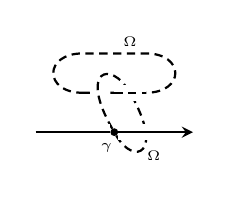
\begin{tikzpicture}
%%loop
\draw[regular] (0.6,0) -- (1.4,0)
	.. controls +(0:0.5cm) and +(0:0.5cm) .. (1.4,0.5)
	-- (0.6,0.5)
	.. controls +(180:0.5cm) and +(180:0.5cm) .. (0.6,0);
\node at (1.2,0.65) {\tiny $\Omega$};
%%gamma loop
\node[dotnode] (ga) at (1,-0.5) {};
\node at (0.9,-0.7) {\tiny $\gamma$};
\draw[overline,regular] (ga)
	.. controls +(120:0.9cm) and +(120:0.5cm) .. (1.2,0)
	.. controls +(-60:0.9cm) and +(-60:0.5cm) .. (ga);
\node at (1.5,-0.8) {\tiny $\Omega$};
%%gamma through line
\draw[overline,->] (0,-0.5) -- (ga) -- (2,-0.5);
\draw[overline,regular] (1,0) -- (1.4,0);
\end{tikzpicture}


%%%%%%%%%%%%%%%%%%%%%%%%%%%%%%%%%%%%%%%%%%%%%%%%%%%%%%%%%%%%%%%%%%%%%%
graphic 15
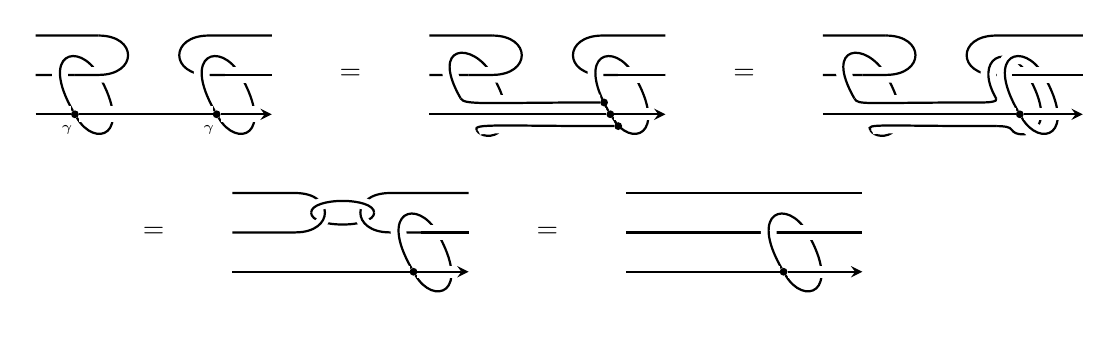
\begin{tikzpicture}
\begin{scope}[shift={(0,0)}]
%%half loop
\draw (0,0) -- (0.8,0)
	.. controls +(0:0.5cm) and +(0:0.5cm) .. (0.8,0.5) -- (0,0.5);
\draw (3,0) -- (2.2,0)
	.. controls +(180:0.5cm) and +(180:0.5cm) .. (2.2,0.5) -- (3,0.5);
%%gamma loops
\node[dotnode] (ga) at (0.5,-0.5) {};
\node[dotnode] (ga2) at (2.3,-0.5) {};
\node at (0.4,-0.7) {\tiny $\gamma$};
\node at (2.2,-0.7) {\tiny $\gamma$};
\draw[overline] (ga)
	.. controls +(120:0.9cm) and +(120:0.5cm) .. (0.8,0)
	.. controls +(-60:0.9cm) and +(-60:0.5cm) .. (ga);
\draw[overline] (ga2)
	.. controls +(120:0.9cm) and +(120:0.5cm) .. (2.6,0)
	.. controls +(-60:0.9cm) and +(-60:0.5cm) .. (ga2);
%%gamma through line
\draw[overline,->] (0,-0.5) -- (ga) -- (ga2) -- (3,-0.5);
%%overline for half loop
\draw[overline] (0.5,0) -- (0.8,0)
	.. controls +(0:0.5cm) and +(0:0.5cm) .. (0.8,0.5);
\draw[overline] (2.4,0) -- (3,0);
\end{scope}
%%%%%%%%%%%%%%%%%%%%%%%
\node at (4,0) {$=$};
%%%%%%%%%%%%%%%%%%%%%%%
\begin{scope}[shift={(5,0)}]
%%half loop
\draw (0,0) -- (0.8,0)
	.. controls +(0:0.5cm) and +(0:0.5cm) .. (0.8,0.5) -- (0,0.5);
\draw (3,0) -- (2.2,0)
	.. controls +(180:0.5cm) and +(180:0.5cm) .. (2.2,0.5) -- (3,0.5);
%%gamma loops
%\node[dotnode] (ga) at (0.5,-0.5) {};
\node[dotnode] (ga2) at (2.3,-0.5) {};
%\node at (0.4,-0.7) {\tiny $\gamma$};
%\node at (2.2,-0.7) {\tiny $\gamma$};
%\draw[overline] (ga)
%	.. controls +(120:0.9cm) and +(120:0.5cm) .. (0.8,0)
%	.. controls +(-60:0.9cm) and +(-60:0.5cm) .. (ga);
\draw[overline] (ga2)
	.. controls +(120:0.9cm) and +(120:0.5cm) .. (2.6,0)
	.. controls +(-60:0.9cm) and +(-60:0.5cm) .. (ga2);
%%gamma loop merged
\node[dotnode] (a1) at (2.22,-0.35) {};
\node[dotnode] (a2) at (2.4,-0.65) {};
\node[emptynode] (x) at (0.4,-0.3) {};
\node[emptynode] (y) at (0.6,-0.7) {};
\draw[overline] (x)
	.. controls +(120:0.8cm) and +(120:0.5cm) .. (0.8,0)
	.. controls +(-60:0.9cm) and +(-60:0.2cm) .. (y);
\draw[overline] (x)
	.. controls +(-60:0.1cm) and +(180:1.5cm) .. (a1);
\draw[overline] (y)
	.. controls +(120:0.1cm) and +(180:1.5cm) .. (a2);
\draw (ga2) -- (a2);
%%gamma through line
\draw[thin_overline={1.5},->] (0,-0.5) -- (ga2) -- (3,-0.5);
%%overline for half loop
\draw[overline] (0.5,0) -- (0.8,0)
	.. controls +(0:0.5cm) and +(0:0.5cm) .. (0.8,0.5);
\draw[overline] (2.4,0) -- (3,0);
\end{scope}
%%%%%%%%%%%%%%%%%%%%%%%%%%%%%%%%
\node at (9,0) {$=$};
%%%%%%%%%%%%%%%%%%%%%%%
\begin{scope}[shift={(10,0)}]
%%half loop
\draw (0,0) -- (0.8,0)
	.. controls +(0:0.5cm) and +(0:0.5cm) .. (0.8,0.5) -- (0,0.5);
\draw (3.3,0) -- (2.2,0)
	.. controls +(180:0.5cm) and +(180:0.5cm) .. (2.2,0.5) -- (3.3,0.5);
%%gamma loops
%\node[dotnode] (ga) at (0.5,-0.5) {};
\node[dotnode] (ga2) at (2.5,-0.5) {};
%\node at (0.4,-0.7) {\tiny $\gamma$};
%\node at (2.2,-0.7) {\tiny $\gamma$};
%\draw[overline] (ga)
%	.. controls +(120:0.9cm) and +(120:0.5cm) .. (0.8,0)
%	.. controls +(-60:0.9cm) and +(-60:0.5cm) .. (ga);
%%gamma loop merged
\node[emptynode] (a1) at (2,-0.35) {};
\node[emptynode] (a2) at (2.2,-0.65) {};
\node[emptynode] (x) at (0.4,-0.3) {};
\node[emptynode] (y) at (0.6,-0.7) {};
\node[emptynode] (x2) at (2.2,-0.3) {};
\node[emptynode] (y2) at (2.4,-0.7) {};
%half loop on the left
\draw[overline] (x)
	.. controls +(120:0.8cm) and +(120:0.5cm) .. (0.8,0)
	.. controls +(-60:0.9cm) and +(-60:0.2cm) .. (y);
%rest of loop
\draw[overline] (x)
	.. controls +(-60:0.1cm) and +(180:1.5cm) .. (a1)
	.. controls +(0:0.1cm) and +(-60:0.05cm) .. (x2)
	.. controls +(120:0.6cm) and +(120:0.5cm) .. (2.6,0)
	.. controls +(-60:0.9cm) and +(-60:0.15cm) .. (y2)
	.. controls +(120:0.05cm) and +(0:0.1cm) .. (a2);
\draw[overline] (y)
	.. controls +(120:0.1cm) and +(180:1.5cm) .. (a2);
%%right gamma loop
\draw[overline] (ga2)
	.. controls +(120:0.9cm) and +(120:0.5cm) .. (2.8,0)
	.. controls +(-60:0.9cm) and +(-60:0.5cm) .. (ga2);
%\draw (ga2) -- (a2);
%%gamma through line
\draw[thin_overline={1.5},->] (0,-0.5) -- (ga2) -- (3.3,-0.5);
%%overline for half loop
\draw[overline] (0.5,0) -- (0.8,0)
	.. controls +(0:0.5cm) and +(0:0.5cm) .. (0.8,0.5);
\draw[overline] (2.4,0) -- (3.3,0);
\end{scope}
%%%%%%%%%%%%%%%%%%%%%%%
\node at (1.5,-2) {$=$};
%%%%%%%%%%%%%%%%%%%%%%%
\begin{scope}[shift={(2.5,-2)}]
%%cross loop, bottom part
\draw (1,0.25)
	.. controls +(-90:0.2cm) and +(-90:0.2cm) .. (1.8,0.25);
%%half loops
\draw[thin_overline={1.5}] (0,0) -- (0.8,0)
	.. controls +(0:0.5cm) and +(0:0.5cm) .. (0.8,0.5) -- (0,0.5);
\draw[thin_overline={1.5}] (3,0) -- (2,0)
	.. controls +(180:0.5cm) and +(180:0.5cm) .. (2,0.5) -- (3,0.5);
%%gamma loops
%\node[dotnode] (ga) at (0.5,-0.5) {};
\node[dotnode] (ga2) at (2.3,-0.5) {};
\draw[overline] (ga2)
	.. controls +(120:0.9cm) and +(120:0.5cm) .. (2.6,0)
	.. controls +(-60:0.9cm) and +(-60:0.5cm) .. (ga2);
%%gamma loop merged
%%gamma through line
\draw[thin_overline={1.5},->] (0,-0.5) -- (ga2) -- (3,-0.5);
%%overline for half loop
\draw[overline] (2.4,0) -- (3,0);
%%overline for cross loop
\draw[thin_overline={1.5}] (1,0.25)
	.. controls +(90:0.2cm) and +(90:0.2cm) .. (1.8,0.25);
\end{scope}
%%%%%%%%%%%%%%%%%%%%%%%
\node at (6.5,-2) {$=$};
%%%%%%%%%%%%%%%%%%%%%%%
\begin{scope}[shift={(7.5,-2)}]
\draw (0,0) -- (3,0);
\draw (0,0.5) -- (3,0.5);
%%gamma loops
\node[dotnode] (ga2) at (2,-0.5) {};
\draw[overline] (ga2)
	.. controls +(120:0.9cm) and +(120:0.5cm) .. (2.3,0)
	.. controls +(-60:0.9cm) and +(-60:0.5cm) .. (ga2);
%%gamma loop merged
%%gamma through line
\draw[thin_overline={1.5},->] (0,-0.5) -- (ga2) -- (3,-0.5);
\draw[overline] (2,0) -- (3,0);
\end{scope}
\end{tikzpicture}
%%%%%%%%%%%%%%%%%%%%%%%%%%%%%%%%%%%%%%%%%%%%%%%%%%%%%%%%%%%%%%%%%%%%%%
%%%%%%%%%%%%%%%%%%%%%%%%%%%%%%%%%%%%%%%%%%%%%%%%%%%%%%%%%%%%%%%%%%%%%%
%%%%%%%%%%%%%%%%%%%%%%%%%%%%%%%%%%%%%%%%%%%%%%%%%%%%%%%%%%%%%%%%%%%%%%
%%%%%%%%%%%%%%%%%%%%%%%%%%%%%%%%%%%%%%%%%%%%%%%%%%%%%%%%%%%%%%%%%%%%%%
\end{document}
